\scanpage{87}
% The writing is upside down in the supplied scan; transcribed in its reading orientation.
% Faint mirrored typescript is show-through from the sheet transcribed as scan 86.
\handwritten{\diagram{\(\begin{array}{ll}
\begin{tikzpicture}[overlay,x=1cm,y=1cm]
\draw[line width=.25pt] (-.17,.6)--(-.19,.27);
\draw[line width=.25pt] (-.2,.2)--(-.22,-.28);
\draw[line width=.25pt] (-.22,-.35) .. controls (-.25,-.65) and (-.25,-.8) .. (-.12,-.92);
\draw[line width=.25pt] (-.1,-.95) .. controls (-.02,-1.02) and (.02,-1.07) .. (.06,-1.1);
\end{tikzpicture}
A_n,\ A_n^{\unsure{\mathrm{ad}|{\cdot}d|-d}},\ (\unsure{A_{n,d}|A_n,d})\quad(d\mid n,\ 1<d<n)
& \widetilde{A}_n,\ \widetilde{A}_n^{\mathrm{ad}},\ (\widetilde{A}_n,d)\ ,\\[.6em]
B_n,\ B_n^{\mathrm{ad}} & \\
C_n,\ C_n^{\mathrm{ad}} & \widetilde{D}_n,\ \widetilde{D}_n^{\mathrm{ad}},\ \widetilde{D}_n^{\unsure{\mathrm{orth}|\mathrm{orb}}}\ ,\\[.6em]
D_n,\ D_n^{\mathrm{ad}},\ \underset{\begin{gathered}\text{\begin{tikzpicture}[x=.15cm,y=.15cm]
\draw (0,1) .. controls (0,.35) and (.1,0) .. (.75,0);
\end{tikzpicture}}\\[-.6ex]\text{orth}\end{gathered}}{D'_n},\ D''_n\quad(\text{si }n\text{ pair }\geq6)
& \widetilde{E}_6,\ \widetilde{E}_6^{\mathrm{ad}}\\[.6em]
E_6\quad E_6^{\mathrm{ad}} & \\
E_7,\ E_7^{\mathrm{ad}} & \\
E_8, & \\
F_4\unsure{.|,} & \\
G_2 &
\end{array}\)}}

\handwritten{\diagram{\(\begin{array}{lcl}
21\ \text{\uline{cas à examiner}} & \left\{\begin{array}{l}
\text{a) en partant des groupes \unsure{compacts connexes gr. de réf.|comp. et ce comme gr. de réf.|compacts connexes gr. de Lie}.}\\[.7em]
\text{b) en partant \unsure{de|des} Chevalley}
\end{array}\right. &
\end{array}\)}}
\handwritten{\figure{\begin{tikzpicture}
\draw (0,0) -- (2.3,.03) -- (4.2,0) -- (6,.035) -- (8,.01) -- (10,.045) -- (12,.15);
\draw[line width=.3pt] (3.3,.13)--(3.4,.13);
\draw[line width=.3pt] (4.12,.16)--(4.28,.18);
\draw[line width=.3pt] (8.12,-2.4) .. controls (8.2,-2.4) and (8.32,-2.45) .. (8.42,-2.47);
\end{tikzpicture}}}
% archive sheet number: 86
